%\documentclass{aghdpl}               % przy kompilacji programem latex
\documentclass[pdflatex,en]{aghdpl}  % praca w języku angielskim
\usepackage[utf8]{inputenc}
\usepackage{float}
\usepackage[dvipsnames]{xcolor}
\usepackage{pdfpages}
\usepackage{ragged2e}

% dodatkowe pakiety
\usepackage{enumerate}
\usepackage{listings}
\usepackage[nottoc]{tocbibind}
%---------------------------------------------------------------------------

\author{Szymon Lenart}
\shortauthor{Sz. Lenart}

\titleEN{Visual Bicycle Counter}

\thesistypeEN{Bachelor of Science Thesis}

\supervisorEN{Mikołaj Leszczuk Ph.D}

\date{2020}

\facultyEN{Faculty of Electrical Engineering, Computer Science and Electronics}

%\acknowledgements{Serdecznie dziękuję \dots tu ciąg dalszych podziękowań np. dla promotora, żony, sąsiada itp.}

\setlength{\cftsecnumwidth}{10mm}

%---------------------------------------------------------------------------

\begin{document}

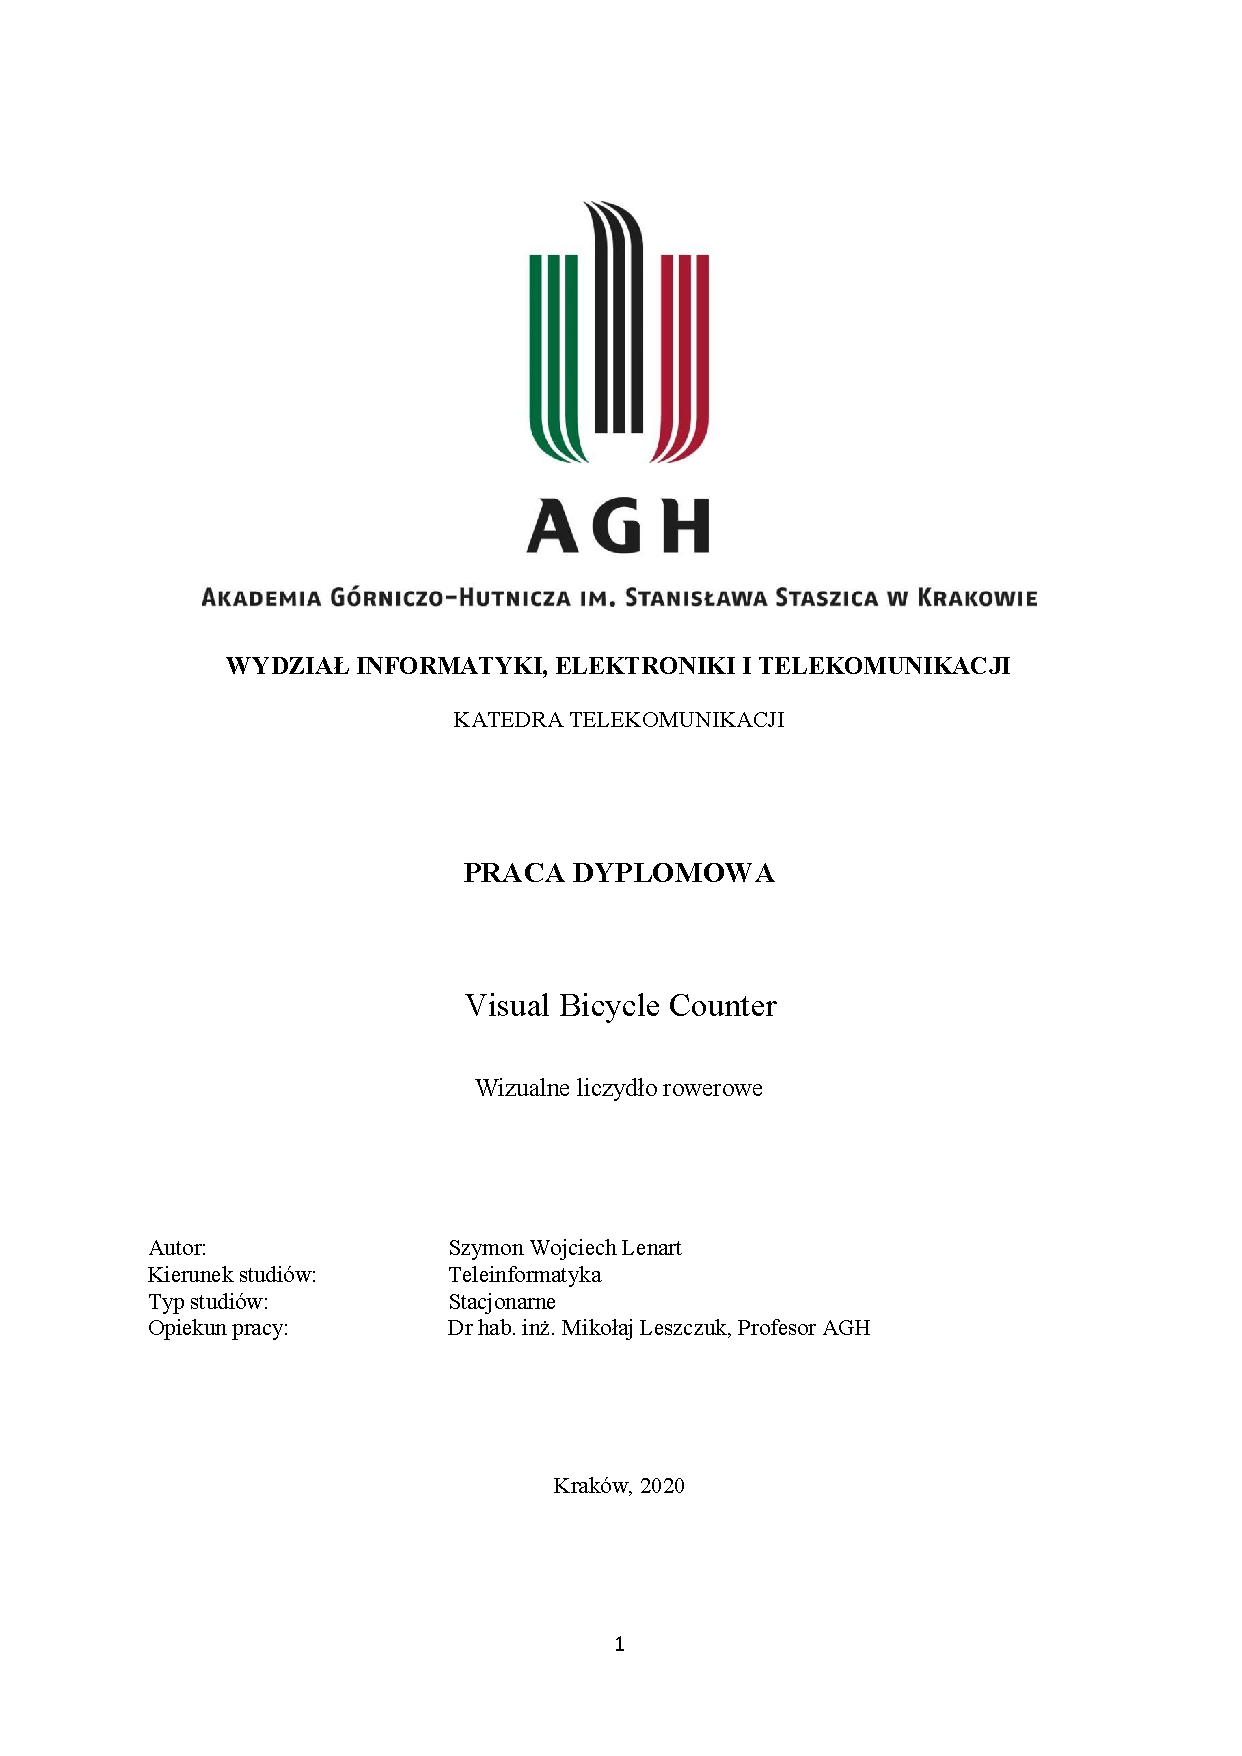
\includepdf[page=-]{title_page}

\begin{flushright}
Serdecznie dziękuję mojej Żonie, za okazane mi wsparcie w trakcie pisania tej pracy.
\end{flushright}

\tableofcontents

\chapter{Introduction}
\label{cha:introduction}

Bicycle counter is a device that automatically counts cyclists riding on the road. Roadside counting devices for riding cyclists are installed in many cities, also in Krakow. They are usually part of the city's broader strategy, wanting to encourage its residents to ride bicycles. The bicycle counter usually works on induction loops embedded in a nearby bicycle path that detect passing bikes. Sometimes photocells are also used to count cyclists. However, this work's scope is to create visual bicycle counters, based on techniques for recognizing images from publicly available webcams. These data should be counted over a longer time horizon, and, optimally, be combined with data on cards from automatic, urban cycling measurement points.

%---------------------------------------------------------------------------

\section{Goals}
\label{sec:goals}

My thesis's goal was to create a mechanism for counting cyclist on the video file, downloaded from publicly available street cameras' view. That, in turn, could help evaluate investments made by city authorities or plan future projects.


%---------------------------------------------------------------------------

\section{My Contribution}
\label{sec:myContribution}

To achieve the mentioned goal, I had to research the newest Machine Learning and Computer Vision algorithms and techniques and learn how to customize their functioning. As an addition, I have not only trained the AI model to detect and count cyclist but also used it on more video files to get data and show good visualization and its interpretation.

%---------------------------------------------------------------------------

\section{Order of content}
\label{sec:orderOfContent}
First of all, I will write about theoretical aspects of my work with \textit{State of the Art} of Computer Vision and Machine Learning in traffic planning and analysis. Then I will describe the practical side of work I had to do to achieve the goals of my thesis. In the end, I would like to show the results of my work as well as the visualization of data my program collects with the exemplary interpretation of this data. 















\chapter{Theoretical aspects}
\label{cha:theorethicalAspects}

In this chapter I would like to describe theory standing behind my work and how is it used nowadays.

%---------------------------------------------------------------------------

\section{State of the Art}
\label{sec:stateOfTheArt}

Nowadays broadly understood data becomes one of the most desired needed resource, everyone wants to make research about everything. For example a lot of mobile applications wants its user to let it access localization or allow it to send some information to servers. But more data we have, the more time it requires from human to process it and extract only things we need. Top it all off it needs to be interpreted afterwards to make some sense of it. That is why Data Science becomes so popular these days. It tries to solve the problem of growing time taken to process bigger and bigger sets of data. The solution turned out to be simple - "let the machines do the work". That is how Machine Learning (ML) was born. Computer Vision (CV) in the other hand is an Artificial Intelligence (AI) branch specified for working with image/video and it uses ML algorithms as a step to achieve its goals of extracting needed data from images/videos with as little human work as possible. As of today CV finds more and more application in various science branches. The most known use of CV is development of Autonomous Driving. There is also technology for monitoring and prevention of pests and grass diseases\cite{appResearch}, based on CV. Also as a example, China's government works on spread of street cameras with face recognition software, but that is less of a positive example as some would say, used for human behaviour control. But in my knowledge there is no Visual Bicycle Counter in commercial application.


%---------------------------------------------------------------------------

\section{What a Bicycle Counter is and why make it "Visual"}
\label{sec:why}

Bicycle Counter, as the name suggest is a device for counting cyclists driving by specific street or bike path. Usually it is a convection loop embedded in asphalt of a road, but photocells installed by the roadside are getting more popular too. Both devices count cyclists passing by and save the number on some sort of server, to make it accessible to obtain for authorized people. Those information can later serve as a good indicator of bicycle traffic in the city. In figure \ref{fig:countersKrakow} we can see that in Krakow there is 17 of those devices installed in across the city and numbers from them are publicly available.
\begin{figure}[H]
    \centering
    \resizebox{\textwidth}{!}{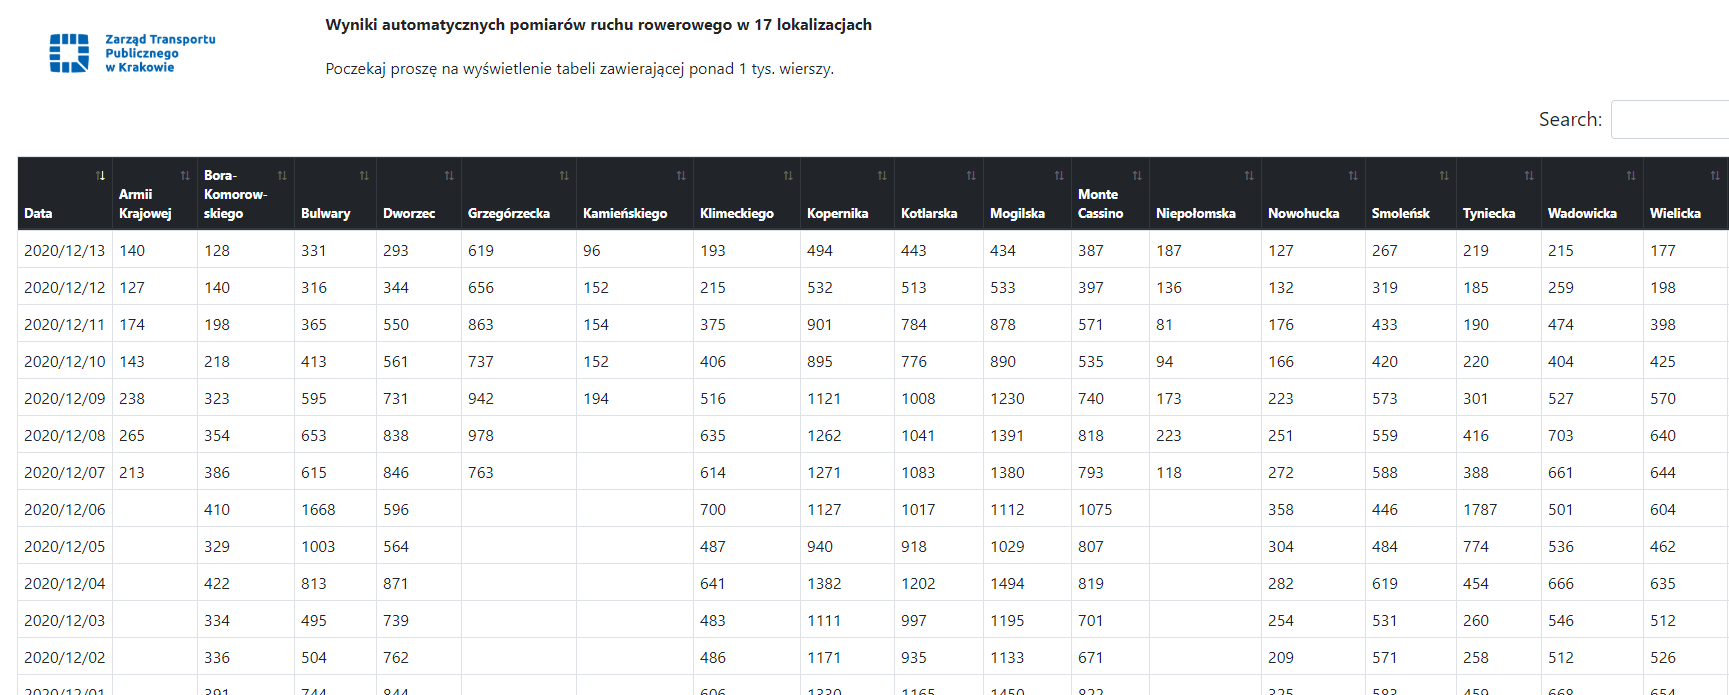
\includegraphics{images/countersKrakow}}
    \caption{First rows of data from bicycle counters installed in Krakow \cite{mobilnykrakow}}
    \label{fig:countersKrakow}
\end{figure}
But why even bother about making Visual Bicycle Counter? First of all, devices I mentioned above are all another equipment used with only one purpose - counting cyclists, so their reusability leaves a lot to be desired. Secondly, installing such a device requires to put more work into it, because you need to for example make a hole in road, put a convection loop in and patch the hole up. Same as maintenance can be problematic too. Visual Bicycle Counter could solve those issues. It uses trained ML model to perform inference on video files from street cameras downloaded on computer or straight on video streams from websites which share it publicly. That would not add next device, but would use existing infrastructure of street cameras, widely developed in many cities.


%---------------------------------------------------------------------------

\section{Short theory behind Visual Bicycle Counter}
\label{sec:theory}

Visual Bicycle Counter bases on deep learning model, what has advantage over traditional target detection. "The traditional method is to manually extract features and require experts in related fields to manually design and process them through years of accumulation and experience. The method of deep learning can learn the features of difference in response data through a large amount of data and is more representative. The deep learning model simulates the human brain's visual perception system. It extracts features directly from the original image, and the features are passed through the layer by layer to obtain the high-dimensional information of the image, making it a great success in the field of computer vision."\cite{deepLearning} But first I had to train my model what consists of collecting data to create a dataset for training (in my case: label video frames - show exactly where cyclist is, divide labelled frames to train and test). Training the model is "showing" computer training data, it learns those and based on what is learns it tries to predict desired information on test data and then process is repeated many, many times until reaching satisfactory parameters. For me, main metrics were: Loss, Recall, Precision. Loss is basically a target function, that is minimized in optimization process (the lower the better and it gets lower when model predicts more accurately). Recall means how many items that should be selected was actually selected, and Precision means how many selected items are actually our desired items. Visualization of Recall and Precision is shown in figure \ref{fig:RPL}.

\begin{figure}[H]
    \centering
    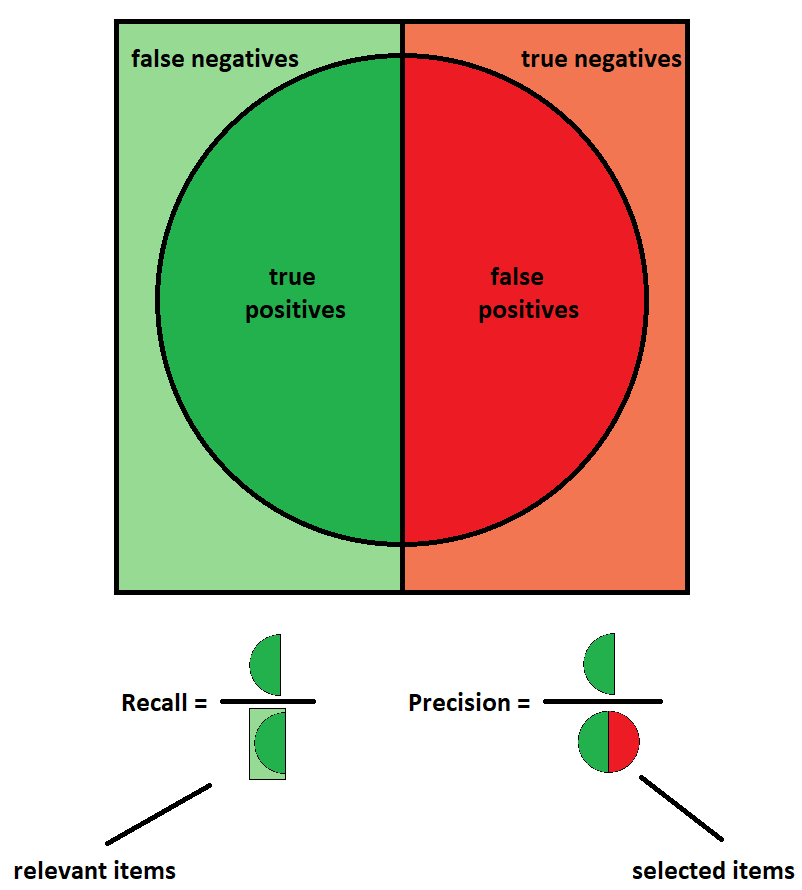
\includegraphics[scale=0.5]{images/rpl}
    \caption{Recall and Precision}
    \label{fig:RPL}
\end{figure}

%---------------------------------------------------------------------------
\section{Tools selection}
\label{sec:tools}

Tools I have used to create my Visual Bicycle Counter were as follow:
\begin{itemize}
    \item youtube-dl software for downloading video streams from street cameras as mp4 files
    \item LabelImg program for manual image labelling 
    \item Virtual Machine with Ubuntu 18.04.5 LTS for download scheduling 
    \item Google Colaboratory as working environment,
    \item Python programming language,
    \item OpenCV libraries for object detection (used by YOLOv5 API),
    \item YOLOv5 API for training YOLO\cite{Redmon_2016_CVPR} models and performing inference,
    \item Wandb for training evaluation.
\end{itemize}
Most of the choices was pretty obvious. I was looking for widely used solutions that provides good documentation and big user base. Youtube-dl was the easiest tool to install and use. Using Google Colaboratory (GC) machine was not only my choice, but at certain stage of work I simply needed more powerful GPU and CPU. GC provided all that as well as Python programming language support. Biggest challenge appeared when I was looking for Object Detection tools. I had to test different solutions, as Tensorflow with Keras, but I found it to be not suitable for my use case so I decided to use OpenCV libraries, YOlOv5 API and Wandb that appeared much more user friendly and provided all features I needed.

\chapter{Practical aspects}
\label{cha:practicalAspects}

To achieve my goal of creating Visual Bicycle Counter, I had to complete a few steps. With tools chosen, my work was to create a proper dataset for training ML model, train and evaluate this training to reach acceptable values of metrics I mentioned in section \ref{sec:theory}. After that, I could customize the API detection script to make it count cyclist rather than just detecting them using the trained model. Lastly, I used my edited script to run inference (detection) on other videos from a street camera on Lema Street, where bike road was modernized in July this year. I used videos before and after modernization, to prepare a simple comparison, as an example of how data obtained by my Visual Bicycle Counter can be used.

\section{Data collection}
\label{sec:collection}
First of all I had to collect data. To accomplish that, at the end of June 2020 I have created Virtual Machine (VM) with Ubuntu 18.04.5 Operating System (OS). Using Unix type OS was much easier and intuitive than using it on my Windows machine. After my VM was ready, steps to obtain video files from street camera stream were as follow:
\begin{enumerate}
    \item Installing ffmpeg for Ubuntu OS(from terminal):
    \begin{itemize}
        \item \colorbox{Gray}{sudo apt-get install ffmpeg}
    \end{itemize}
    \item Downloading and installing youtube-dl (from terminal):
    \begin{itemize}
        \item \colorbox{Gray}{sudo curl -L https://yt-dl.org/downloads/latest/youtube-dl -o /usr/local/bin/youtube-dl}
        \item \colorbox{Gray}{sudo chmod a+rx /usr/local/bin/youtube-dl}
    \end{itemize}
    \item Creating bash script that runs youtube-dl with proper parameters what is shown in figure \ref{fig:script}
    \begin{figure}[H]
        \centering
        \resizebox{\textwidth}{!}{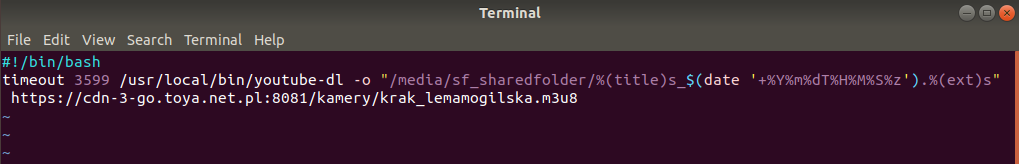
\includegraphics{images/bashScript}}
        \caption{This script runs youtube-dl, video files are saved to  directory with name containing stream name on http website and date of download. After 3599 seconds youtube-dl gets terminated.}
        \label{fig:script}
    \end{figure}
    \item Adding created script to \colorbox{Gray}{crontab -e} to schedule its execution to every hour as we can see in figure below.
    \begin{figure}[H]
        \centering
        \resizebox{\textwidth}{!}{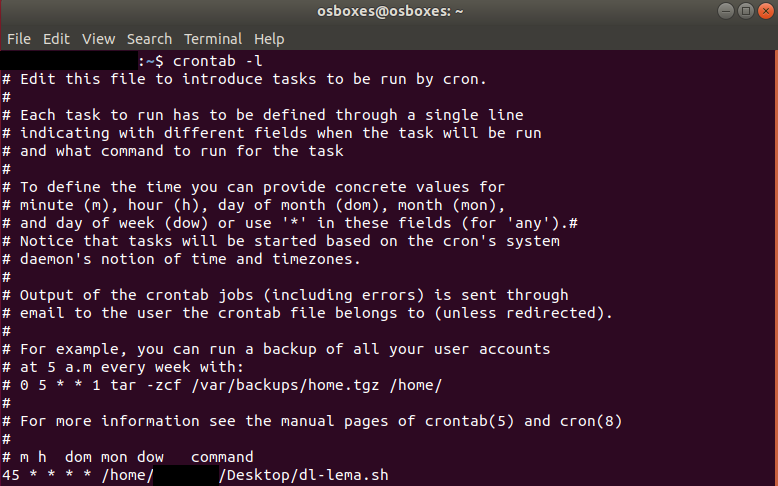
\includegraphics{images/crontabList}}
        \caption{output of \colorbox{Gray}{crontab -l} command which shows what commands execution was scheduled}
        \label{fig:crontabList}
    \end{figure}
\end{enumerate}
At this moment, downloading of video files proceeded automatically. Note that stable internet connection was very important as without it downloaded video files came out corrupted (damaged), what made them impossible to use later on.

\section{Creating the dataset}
\label{sec: dataset}
After collecting enough videos I have started to create the dataset for training my YOLO model. This involved extracting frames from videos, choosing those with the most clear, visible cyclists, then manually labelling each image using LabelImg program and lastly divide labelled images on train and test data in ratio of approximately 8:2. To make it precise, those are steps I have taken:
\begin{enumerate}
    \item Frame extraction with VLC media player
    \begin{itemize}
        \item Scene Filter settings customization
        \newline \colorbox{Gray}{Tools -> Preferences -> Show settings -> All -> Video/Filters/Scene Filter}
        \begin{figure}[H]
            \centering
            \resizebox{\textwidth}{!}{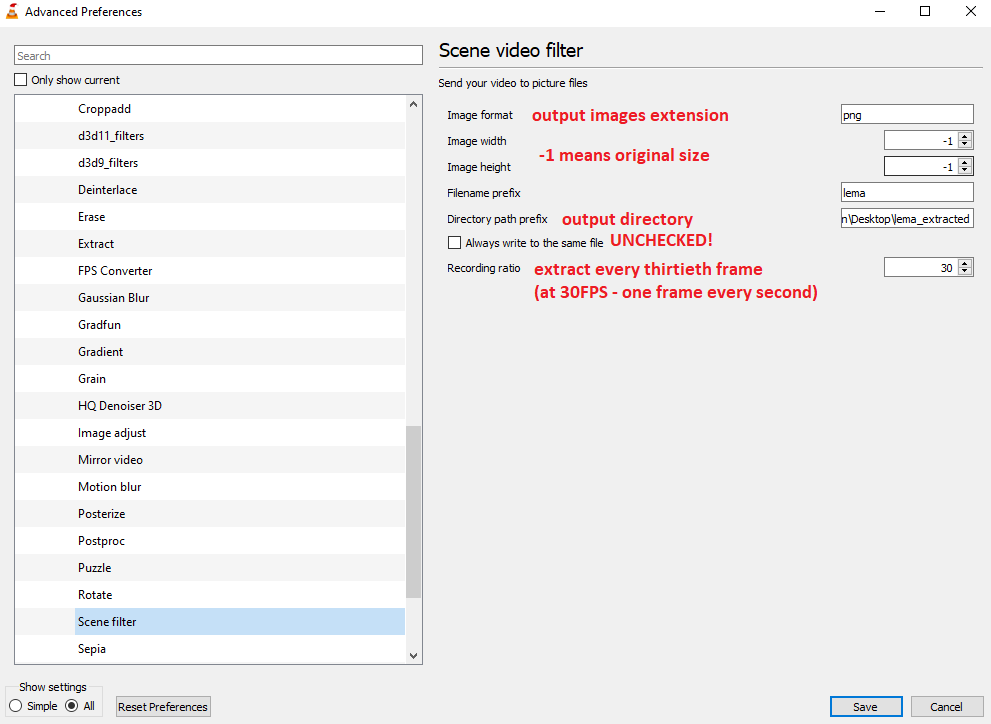
\includegraphics{images/vlc1}}
            \caption{Scene Filter edit window}
            \label{fig:vlc1}
        \end{figure}
        \item Switching Scene filter on
        \newline \colorbox{Gray}{Tools -> Preferences -> Show settings -> All -> Video/Filters -> check Scene video filter}
        \item Restart VLC and run video file with it (at this point frames are extracted automatically) 
    \end{itemize}
    \item Selection of frames (I used about 200 different frames with various count of cyclists on them)
    \item Manual frames labelling using LabelImg:
    \begin{itemize}
        \item after downloading LabelImg from repository, running it by executing command \colorbox{Gray}{python labelImg.py <images-path>} (Python3 or higher required) window shown in figure \ref{fig:labelimg1} appears. It shows labelled image as well. To create label we simply click 
\includegraphics[scale=0.75]{images/button}
        \begin{figure}[H]
            \centering
            \resizebox{\textwidth}{!}{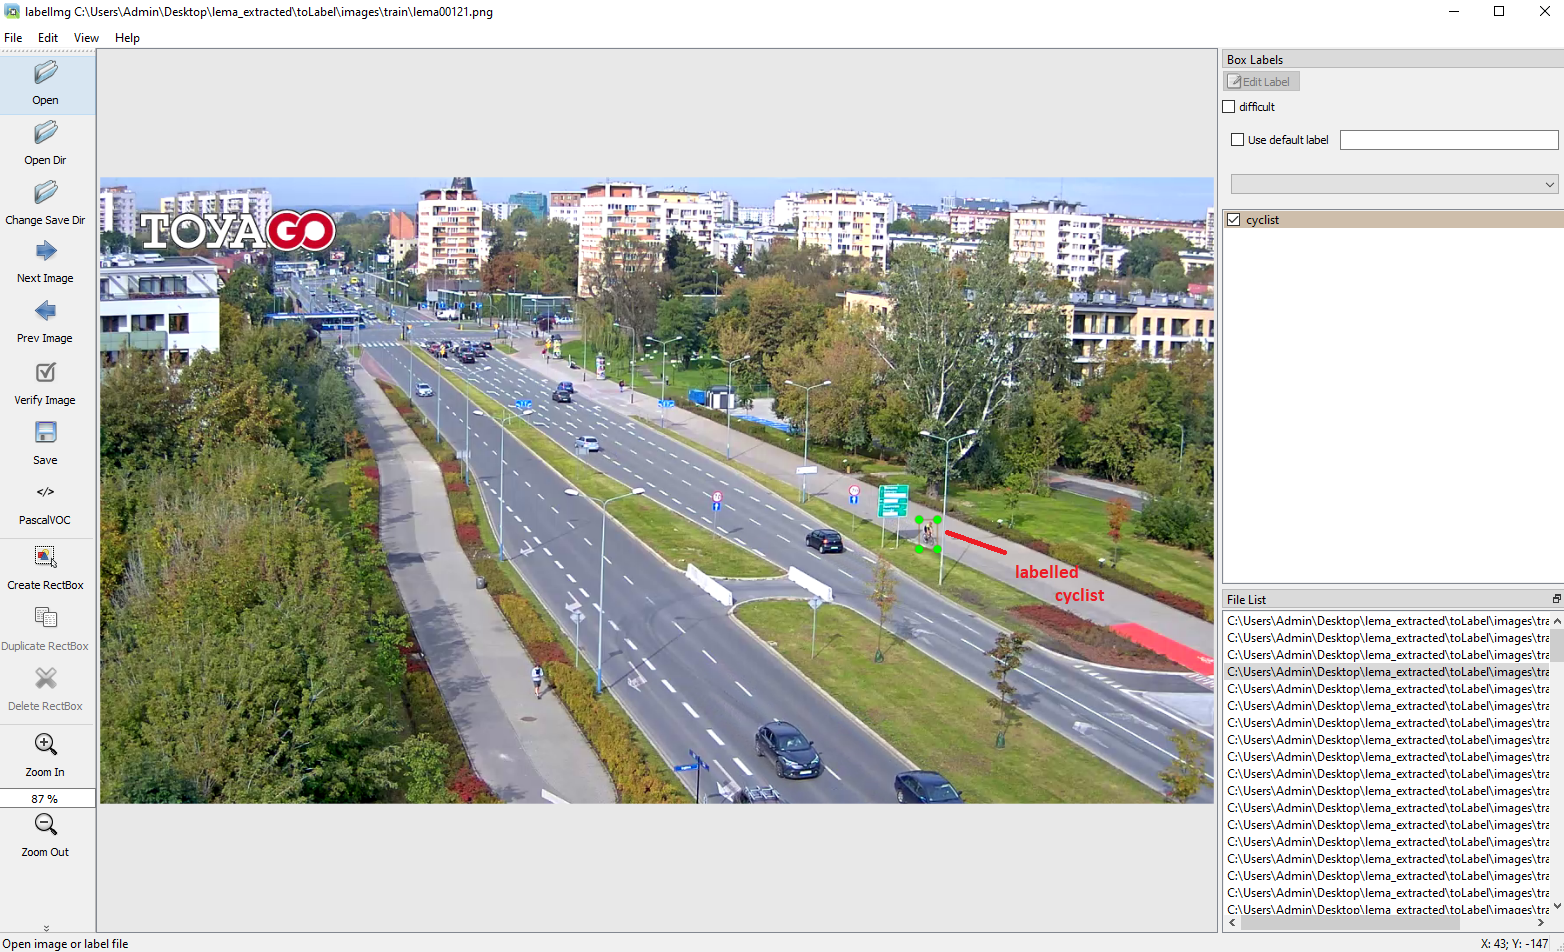
\includegraphics{images/labelImg}}
            \caption{LabelImg user interface with labelled image}
            \label{fig:labelimg1}
        \end{figure}
        Saving labelled frame will generate text file for this image with numeric label representation (one line in file for each label on image).
        \begin{figure}[H]
            \centering
            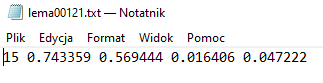
\includegraphics{images/text}
            \caption{Text file generated for image in figure \ref{fig:labelimg1}}
            \label{fig:labelimg2}
        \end{figure}
    \end{itemize}
    \item Partition of images and corresponding text files on train and test (val) data. To accomplish and to do this easier I have written Python script which randomly divides images with text files to two directories "train" and "val" in desired ratio (in my case it was 80\% to train the model and 20\% to test it)
\end{enumerate}

\section{Environment preparation, training model and running detection}
\label{sec:env}
As my working environment, I have chosen Google Colaboratory (GC) machine. It provides me with three times more GPU memory and overall better (faster) GPU device than the one in my computer, resulting in approximately six times faster training and detection processes. It was essential while performing inference (detection) because GC's machine-made this operation execute close to real-time on 30 Frames Per Second (FPS) video files. My computer-processed five frames per second while GC's machine processed almost 30 frames per second, what saved much time. Also, it turned out much more effective while running inference straight on the video stream from the website. Lastly, GC's machine has good Python3 support what facilitated the work. I have created Jupyter Notebook file to run code cells one by one, to speed up my work, what came especially handy while starting work on next day because sadly GC allows only a few hours of inactivity before restarting session and unsaved files are gone. To start training, I stored all necessary files like videos and labelled images on my Google Drive, connected to GC's machine. Also uploading files on the Drive and copying them on the machine was the fastest way to access my computer files. Training the model proceeded in few steps (figures below will show code cells that have been run):
\begin{enumerate}
    \item After setting \colorbox{Gray}{runtime type} to GPU I mounted (connected) my Google Drive to GC's machine what creates a new directory on the machine named \colorbox{Gray}{gdrive} from which we can access Google Drive
    \newline \begin{figure} [h]
        \centering
        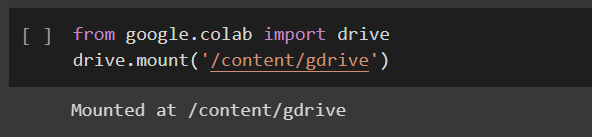
\includegraphics{images/train1}
        \caption{Mounting Drive}
        \label{fig:train1}
    \end{figure}
    \item Then I cloned YoloV5 GitHub repository
    \newline \begin{figure} [h]
        \centering
        \resizebox{\textwidth}{!}{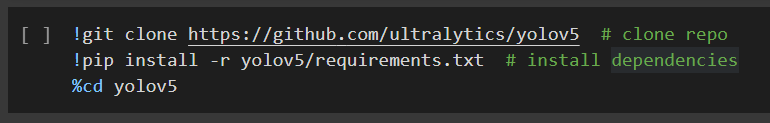
\includegraphics{images/train2}}
        \caption{Cloning repository to machine}
        \label{fig:train2}
    \end{figure}
    \item After that, I could run the training process with installed wandb for evaluating the model during and after training.
    \newline \begin{figure} [h]
        \centering
        \resizebox{\textwidth}{!}{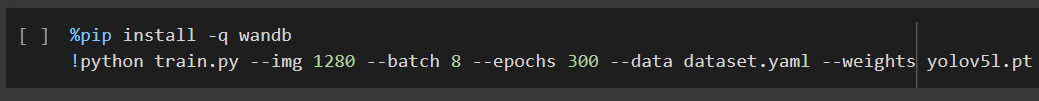
\includegraphics{images/train3}}
        \caption{Command used for training the model}
        \label{fig:train3}
    \end{figure}
    \newline Parameters used in command:
    \begin{itemize}
        \item img - bigger of two numbers in video resolution
        \item batch - how many images to process at once (limited by GPU memory - in my case 8 was the biggest GPU could handle)
        \item epochs - how many times to train the model on whole dataset
        \item data - path to .yaml file which contains information about dataset
        \item weights - path to weights file - empty for training from scratch, I used pretrained weights of yolov5l model, which offers the best accuracy within my desired execution time (<40ms).
    \end{itemize}
\end{enumerate}

\section{Training Evaluation}
\label{sec:eval}
The first command from figure \ref{fig:train3} installs wandb software on the machine. It automatically collects data during the training process and shows it in a more accessible manner - charts. Below we can see how parameters mentioned in section \ref{sec:theory} (Recall, Precision and Loss) has been changing during the training process. Also, weights with the best combination of those three parameters (marked on charts) will be used for performing inference.
\begin{figure} [h]
    \centering
     \resizebox{\textwidth}{!}{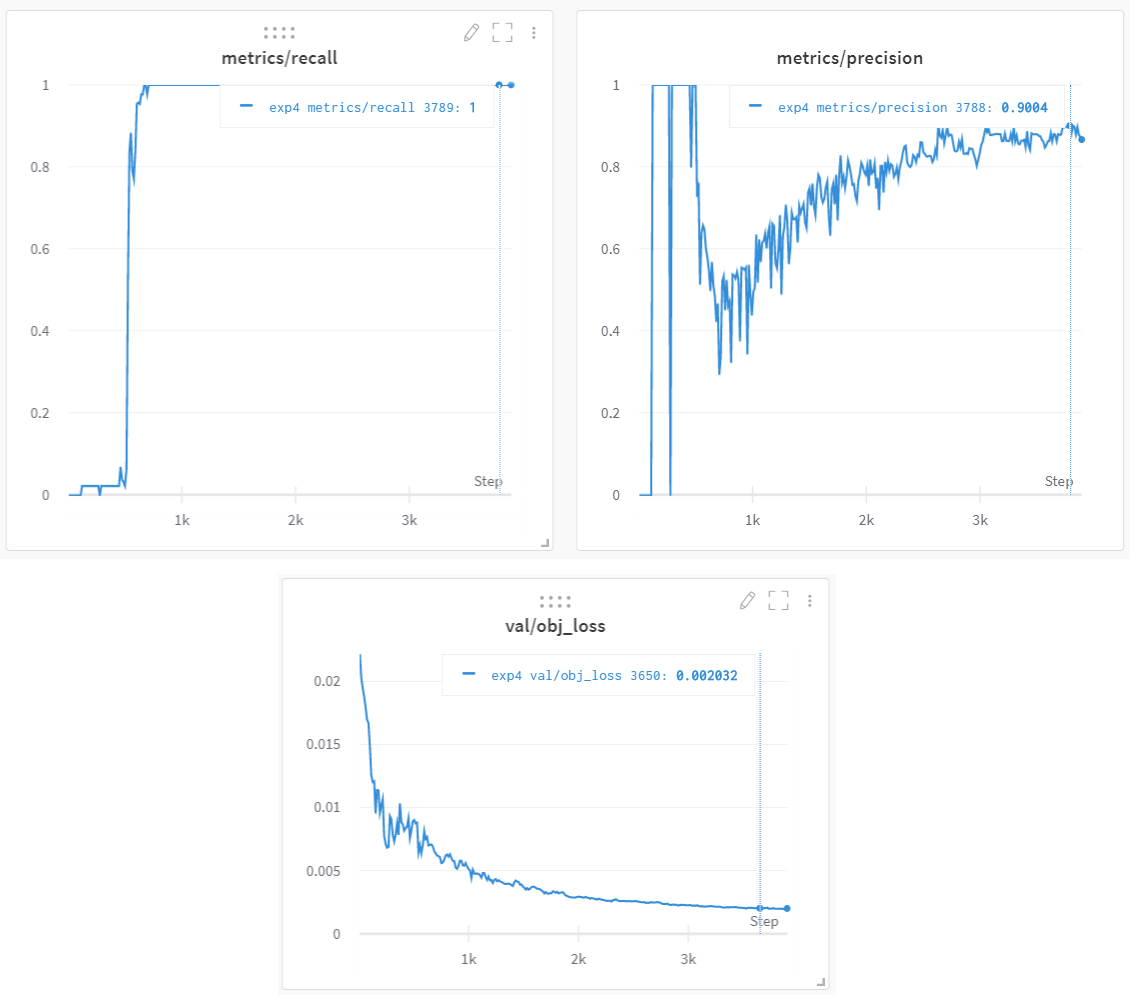
\includegraphics{images/eval1}}
    \caption{Changes of Recall, Precision and Loss during model training}
    \label{fig:eval1}
\end{figure}
\newline As we can see, parameters of trained model I have been using while performing inference on video files I have collected look as follows:
\begin{center}
    \begin{tabular}{ccc}
    Recall    & Precision     & Loss     \\
    1 (100\%) & 0.9004 (90\%) & 0.002032
    \end{tabular}
\end{center}
What basically means that every cyclist on test images was found (Recall), and 90\% of all detections are indeed cyclists (Precision). Also our model finds areas where detection is the most probable with very fast (Loss).

\section{Counter implementation and running inference}
\label{sec:inference}
Running detection process is also really easy with YOLOv5 API, because it contains ready to use script \colorbox{Gray}{detect.py} that can be executed right away on video file or stream. Implementing counter was more of a challenge, because it is not implemented in API. I have chosen straight forward solution - when a detected cyclist crosses a virtual line, counter value goes up. This approach was possible because of my Recall and Precision being on very good level. I knew every cyclist is detected on every frame of video (100\% Recall) and 90\% of detected objects are actually cyclists (Precision). Every script I have customized is put on public Github Repository\cite{repo}. Running detection process on GC's machine proceeded as follows:
\begin{enumerate}
    \item Mounting Google Drive on GC's machine
    \newline \begin{figure} [h]
        \centering
        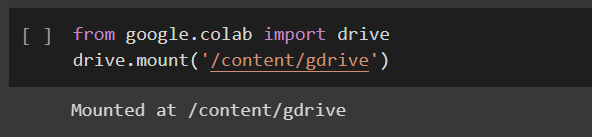
\includegraphics{images/train1}
        \caption{Mounting Drive}
        \label{fig:inference0}
    \end{figure}
    \item Copying model from Drive, unzipping it and installing required dependencies 
    \newline \begin{figure} [h]
        \centering
        \resizebox{\textwidth}{!}{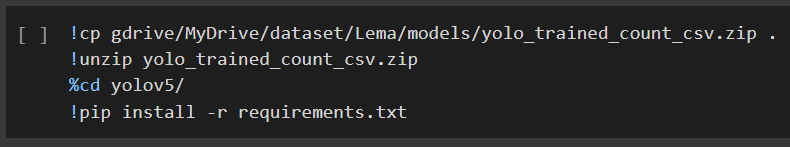
\includegraphics{images/inference1}}
        \caption{Installing ready API on machine}
        \label{fig:inference1}
    \end{figure}
    \item Uploading video for perform inference on it (two ways)
    \newline \begin{figure} [h]
        \centering
         \resizebox{\textwidth}{!}{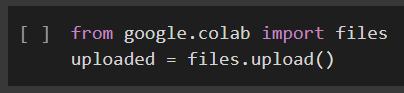
\includegraphics{images/inference2}}
        \caption{Uploading video file straight from local machine to GC's machine (slower)}
        \label{fig:inference2}
    \end{figure}
    \newline \begin{figure} [h]
        \centering
         \resizebox{\textwidth}{!}{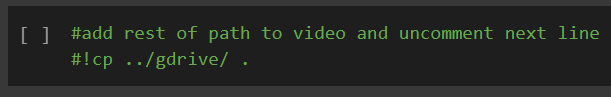
\includegraphics{images/inference3}}
        \caption{Copying video file from mounted drive after uploading video file to it (faster)}
        \label{fig:inference3}
    \end{figure}
    \item Running detection process
    \newline \begin{figure} [h]
        \centering
         \resizebox{\textwidth}{!}{
\includegraphics{images/inference4}}
        \caption{Command used for performing inference on video file using customized \colorbox{Gray}{detect.py} script}
        \label{fig:inference4}
    \end{figure}
    \newline Parameters used in command:
    \begin{itemize}
        \item img - bigger of two numbers in video resolution
        \item source - path to video file
        \item weights - path to weights file (\colorbox{Gray}{best.pt} are best weights from training model) basically it is path to model we will use to detect cyclist
        \item classes - identifier of detection classes to not filter out (\colorbox{Gray}{15} means that we only want to detect cyclists)
        \item conf - confidence threshold value (probability that detected object is indeed cyclist) - everything with higher confidence is considered as cyclist.
    \end{itemize}
\end{enumerate}
The figure below shows a frame from a video on which inference was performed (with Counter already implemented).
\begin{figure} [h]
    \centering
     \resizebox{\textwidth}{!}{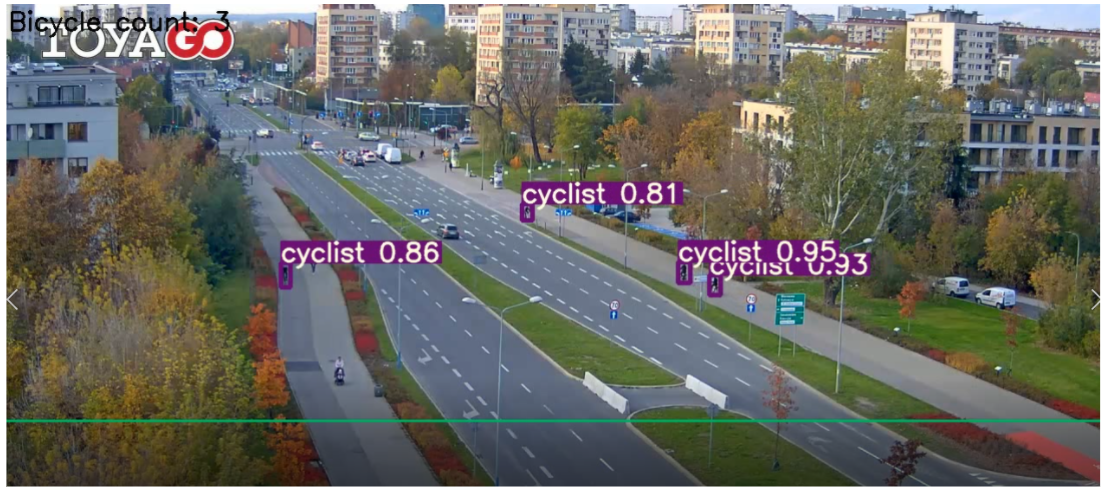
\includegraphics{images/inference}}
    \caption{Frame from video file generated during the detection process}
    \label{fig:inference}
\end{figure}
During the testing phase, I have been saving every video generated during the inference process. However, after that I quit doing that, because a generated video was almost five times bigger than the original one (1-hour video downloaded from website video stream was approximately 700MB big, so saving every result of inference would fill my Google Drive memory very quickly). Instead, I have implemented that at the end of execution of \colorbox{Gray}{detect.py} information about the video was written to \colorbox{Gray}{result.csv} file (video name, video duration, cyclist count).
\section{Exemplary evaluation of results}
\label{sec:results}
To familiarize with the potential of Visual Bicycle Counter, I have prepared an exemplary interpretation of the Counter's data. I had chosen video files collected between 10 AM and 8 PM from a random week before modernization of bike road on Lema Street and performed inference on them. The same I have done with videos from the random week after modernization. This is how the collected data looks like graphically:
\begin{figure} [h]
    \centering
     \resizebox{\textwidth}{!}{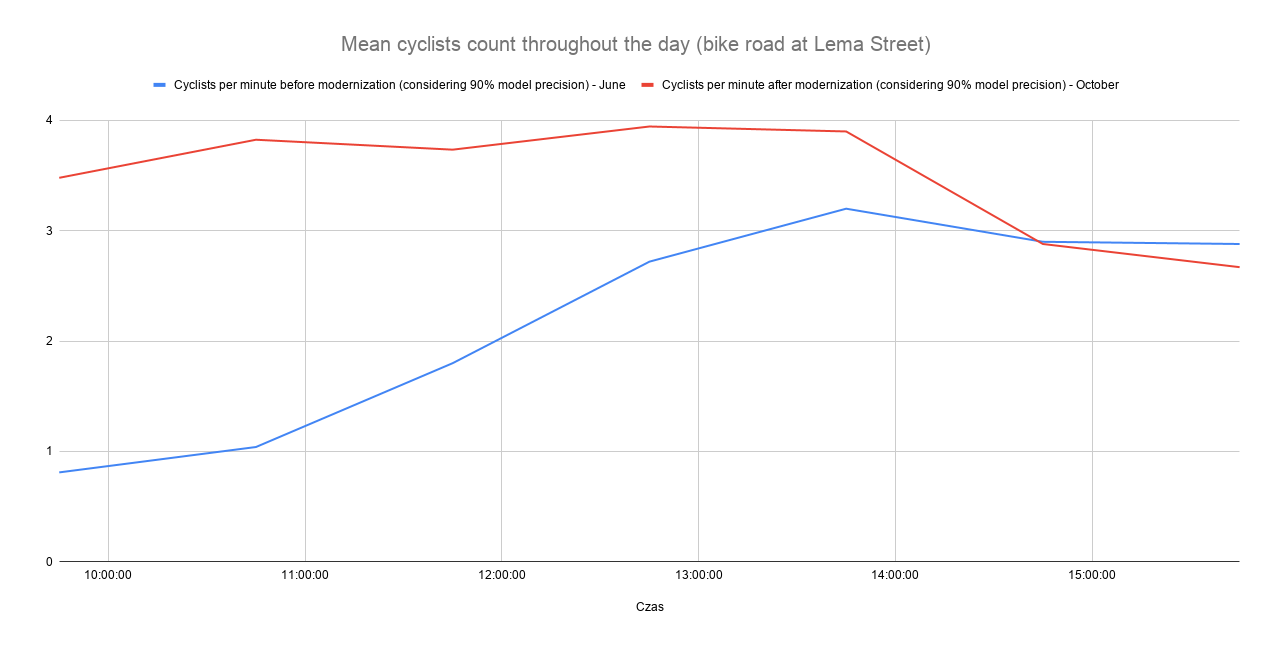
\includegraphics{images/graph}}
    \label{fig:graph}
\end{figure}
Even this simple example provides important information on whether investment turned out to be a success or not. We can see that even though data after modernization was collected in October - the month we cannot call cyclists favourite - number of cyclist per minute was higher than in June. It could be one of the ways to evaluate local government's projects.
\chapter{Exemplary Evaluation of Results}
\label{cha:results}
To familiarize with the potential of Visual Bicycle Counter, I have prepared an exemplary interpretation of the Counter's data. I have been collecting video files from two street cameras - one near ICE Krakow Congress Centre and second on Lema Street. Figure \ref{fig:map} shows those cameras' position on map of Krakow.
\begin{figure}[H]
    \centering
    \resizebox{\textwidth}{!}{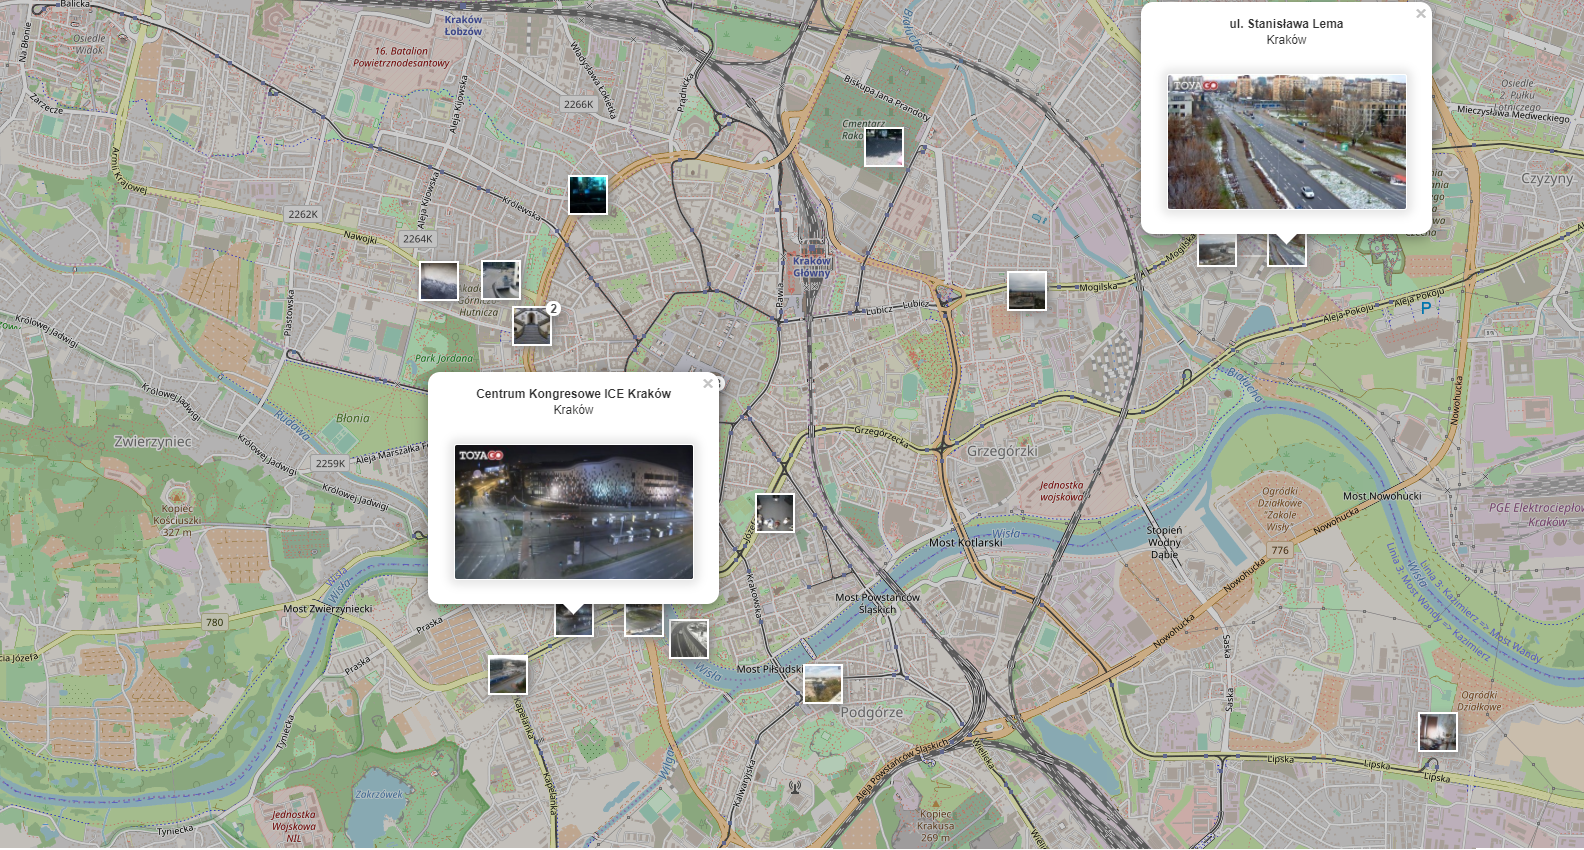
\includegraphics{images/map}}
    \caption{Position of cameras data below comes from\cite{mapa}}
    \label{fig:map}
\end{figure}
For first example I had chosen video files collected between 8:30 AM and 6:30 PM on June and September on bike road near ICE Krakow Congress Centre and performed inference on them. Tables \ref{tab:iceCountJune} and \ref{tab:iceCountSeptember} shows collected cyclists count. Table \ref{tab:iceDaily} aggregates this data to show number of cyclists per day of both months.
\begin{table}[H]
\centering
\resizebox{\textwidth}{!}{
\begin{tabular}{|r|r|r|r|r|r|r|r|r|r|r|}
\hline
\multicolumn{1}{|l|}{} & \multicolumn{10}{c|}{Cyclist count throughout the day (June)}                                                                                                                                                                                                                                                                                            \\ \hline
\multicolumn{1}{|l|}{} & \multicolumn{1}{l|}{8:30-9:30} & \multicolumn{1}{l|}{9:30-10:30} & \multicolumn{1}{l|}{10:30-11:30} & \multicolumn{1}{l|}{11:30-12:30} & \multicolumn{1}{l|}{12:30-13:30} & \multicolumn{1}{l|}{13:30-14:30} & \multicolumn{1}{l|}{14:30-15:30} & \multicolumn{1}{l|}{15:30-16:30} & \multicolumn{1}{l|}{16:30-17:30} & \multicolumn{1}{l|}{17:30-18:30} \\ \hline
1.                     & 307                            & 404                             & 308                              & 302                              & 428                              & 221                              & 98                               & 235                              & 207                              & 239                              \\ \hline
2.                     & 357                            & 313                             & 291                              & 196                              & 214                              & 198                              & 332                              & 141                              & 60                               & 82                               \\ \hline
3.                     & 148                            & 337                             & 479                              & 47                               & 390                              & 330                              & 401                              & 132                              & 78                               & 374                              \\ \hline
4.                     & 364                            & 62                              & 370                              & 288                              & 301                              & 510                              & 467                              & 110                              & 420                              & 103                              \\ \hline
5.                     & 82                             & 45                              & 98                               & 237                              & 138                              & 127                              & 170                              & 50                               & 152                              & 199                              \\ \hline
6.                     & 472                            & 210                             & 120                              & 417                              & 32                               & 306                              & 492                              & 377                              & 265                              & 572                              \\ \hline
7.                     & 251                            & 250                             & 142                              & 372                              & 38                               & 352                              & 225                              & 62                               & 119                              & 83                               \\ \hline
8.                     & 56                             & 124                             & 134                              & 46                               & 71                               & 148                              & 41                               & 389                              & 440                              & 130                              \\ \hline
9.                     & 261                            & 66                              & 154                              & 397                              & 240                              & 73                               & 298                              & 371                              & 103                              & 214                              \\ \hline
10.                    & 179                            & 85                              & 374                              & 96                               & 243                              & 182                              & 52                               & 187                              & 150                              & 328                              \\ \hline
11.                    & 259                            & 244                             & 333                              & 251                              & 321                              & 326                              & 135                              & 190                              & 205                              & 121                              \\ \hline
12.                    & 364                            & 225                             & 282                              & 169                              & 164                              & 320                              & 117                              & 153                              & 168                              & 91                               \\ \hline
13.                    & 273                            & 72                              & 108                              & 265                              & 301                              & 56                               & 126                              & 298                              & 275                              & 343                              \\ \hline
14.                    & 140                            & 95                              & 124                              & 55                               & 171                              & 237                              & 147                              & 159                              & 327                              & 364                              \\ \hline
15.                    & 386                            & 269                             & 224                              & 374                              & 137                              & 139                              & 307                              & 98                               & 323                              & 419                              \\ \hline
16.                    & 246                            & 85                              & 51                               & 337                              & 281                              & 172                              & 87                               & 359                              & 275                              & 74                               \\ \hline
17.                    & 73                             & 197                             & 176                              & 98                               & 275                              & 49                               & 400                              & 84                               & 212                              & 110                              \\ \hline
18.                    & 88                             & 198                             & 202                              & 344                              & 110                              & 143                              & 289                              & 77                               & 321                              & 272                              \\ \hline
19.                    & 85                             & 23                              & 266                              & 192                              & 79                               & 171                              & 217                              & 270                              & 34                               & 235                              \\ \hline
20.                    & 269                            & 44                              & 148                              & 305                              & 22                               & 296                              & 110                              & 192                              & 144                              & 222                              \\ \hline
21.                    & 123                            & 105                             & 57                               & 101                              & 174                              & 15                               & 27                               & 52                               & 102                              & 85                               \\ \hline
22.                    & 62                             & 72                              & 143                              & 195                              & 10                               & 122                              & 87                               & 173                              & 137                              & 28                               \\ \hline
23.                    & 382                            & 136                             & 485                              & 435                              & 315                              & 194                              & 264                              & 535                              & 273                              & 320                              \\ \hline
24.                    & 183                            & 89                              & 342                              & 280                              & 164                              & 92                               & 364                              & 222                              & 292                              & 266                              \\ \hline
25.                    & 297                            & 423                             & 340                              & 41                               & 381                              & 191                              & 48                               & 417                              & 355                              & 470                              \\ \hline
26.                    & 471                            & 137                             & 268                              & 115                              & 304                              & 107                              & 86                               & 364                              & 210                              & 243                              \\ \hline
27.                    & 70                             & 109                             & 363                              & 109                              & 207                              & 176                              & 242                              & 314                              & 212                              & 395                              \\ \hline
28.                    & 197                            & 331                             & 111                              & 158                              & 264                              & 261                              & 485                              & 425                              & 109                              & 410                              \\ \hline
29.                    & 154                            & 236                             & 26                               & 252                              & 103                              & 226                              & 214                              & 189                              & 60                               & 141                              \\ \hline
30.                    & 362                            & 108                             & 404                              & 416                              & 413                              & 517                              & 494                              & 351                              & 388                              & 92                               \\ \hline
\end{tabular}}
\caption{Cyclists count collected from street camera at bike road near ICE Krakow Congress Centre - June}
\label{tab:iceCountJune}
\end{table}
\begin{table}[H]
\centering
\resizebox{\textwidth}{!}{
\begin{tabular}{|r|r|r|r|r|r|r|r|r|r|r|}
\hline
\multicolumn{1}{|l|}{} & \multicolumn{10}{c|}{Cyclist count throughout the day (September)}                                                                                                                                                                                                                                                                                       \\ \hline
\multicolumn{1}{|l|}{} & \multicolumn{1}{l|}{8:30-9:30} & \multicolumn{1}{l|}{9:30-10:30} & \multicolumn{1}{l|}{10:30-11:30} & \multicolumn{1}{l|}{11:30-12:30} & \multicolumn{1}{l|}{12:30-13:30} & \multicolumn{1}{l|}{13:30-14:30} & \multicolumn{1}{l|}{14:30-15:30} & \multicolumn{1}{l|}{15:30-16:30} & \multicolumn{1}{l|}{16:30-17:30} & \multicolumn{1}{l|}{17:30-18:30} \\ \hline
1.                     & 78                             & 138                             & 71                               & 126                              & 174                              & 153                              & 157                              & 10                               & 73                               & 36                               \\ \hline
2.                     & 326                            & 294                             & 288                              & 127                              & 211                              & 93                               & 105                              & 461                              & 258                              & 110                              \\ \hline
3.                     & 540                            & 400                             & 237                              & 353                              & 102                              & 154                              & 340                              & 323                              & 439                              & 270                              \\ \hline
4.                     & 128                            & 106                             & 278                              & 359                              & 550                              & 161                              & 88                               & 305                              & 144                              & 619                              \\ \hline
5.                     & 284                            & 210                             & 588                              & 302                              & 188                              & 481                              & 317                              & 127                              & 109                              & 182                              \\ \hline
6.                     & 147                            & 74                              & 58                               & 54                               & 121                              & 57                               & 10                               & 164                              & 159                              & 79                               \\ \hline
7.                     & 222                            & 62                              & 183                              & 78                               & 216                              & 24                               & 180                              & 121                              & 215                              & 49                               \\ \hline
8.                     & 297                            & 498                             & 262                              & 254                              & 243                              & 422                              & 476                              & 467                              & 128                              & 56                               \\ \hline
9.                     & 439                            & 571                             & 13                               & 378                              & 531                              & 535                              & 242                              & 164                              & 421                              & 146                              \\ \hline
10.                    & 454                            & 420                             & 413                              & 255                              & 142                              & 291                              & 117                              & 257                              & 80                               & 99                               \\ \hline
11.                    & 58                             & 252                             & 126                              & 245                              & 477                              & 438                              & 213                              & 441                              & 295                              & 412                              \\ \hline
12.                    & 221                            & 361                             & 403                              & 220                              & 324                              & 217                              & 255                              & 47                               & 231                              & 367                              \\ \hline
13.                    & 201                            & 448                             & 331                              & 225                              & 94                               & 240                              & 436                              & 326                              & 283                              & 171                              \\ \hline
14.                    & 556                            & 256                             & 180                              & 376                              & 422                              & 154                              & 545                              & 64                               & 399                              & 306                              \\ \hline
15.                    & 485                            & 354                             & 539                              & 100                              & 48                               & 112                              & 442                              & 440                              & 633                              & 271                              \\ \hline
16.                    & 108                            & 306                             & 603                              & 404                              & 490                              & 127                              & 606                              & 122                              & 383                              & 374                              \\ \hline
17.                    & 555                            & 58                              & 268                              & 488                              & 125                              & 87                               & 35                               & 251                              & 241                              & 309                              \\ \hline
18.                    & 281                            & 387                             & 263                              & 413                              & 258                              & 186                              & 262                              & 120                              & 135                              & 117                              \\ \hline
19.                    & 155                            & 184                             & 138                              & 280                              & 257                              & 106                              & 164                              & 300                              & 224                              & 326                              \\ \hline
20.                    & 424                            & 331                             & 406                              & 279                              & 17                               & 372                              & 119                              & 23                               & 108                              & 58                               \\ \hline
21.                    & 227                            & 375                             & 202                              & 365                              & 131                              & 394                              & 184                              & 229                              & 381                              & 307                              \\ \hline
22.                    & 282                            & 302                             & 273                              & 458                              & 433                              & 439                              & 116                              & 449                              & 129                              & 360                              \\ \hline
23.                    & 393                            & 304                             & 274                              & 283                              & 378                              & 413                              & 284                              & 343                              & 168                              & 111                              \\ \hline
24.                    & 419                            & 525                             & 525                              & 146                              & 89                               & 325                              & 508                              & 129                              & 120                              & 45                               \\ \hline
25.                    & 101                            & 168                             & 258                              & 381                              & 353                              & 191                              & 59                               & 384                              & 114                              & 27                               \\ \hline
26.                    & 143                            & 152                             & 11                               & 186                              & 74                               & 40                               & 9                                & 136                              & 36                               & 180                              \\ \hline
27.                    & 112                            & 26                              & 116                              & 41                               & 169                              & 176                              & 86                               & 116                              & 11                               & 249                              \\ \hline
28.                    & 139                            & 227                             & 156                              & 73                               & 105                              & 248                              & 48                               & 5                                & 22                               & 244                              \\ \hline
29.                    & 234                            & 207                             & 168                              & 187                              & 201                              & 160                              & 246                              & 41                               & 76                               & 218                              \\ \hline
30.                    & 105                            & 62                              & 72                               & 12                               & 78                               & 105                              & 38                               & 42                               & 95                               & 117                              \\ \hline
\end{tabular}}
\caption{Cyclists count collected from street camera at bike road near ICE Krakow Congress Centre - September}
\label{tab:iceCountSeptember}
\end{table}
\begin{table}[H]
\centering
\begin{tabular}{|r|r|r|}
\hline
\multicolumn{1}{|l|}{}                 & \multicolumn{2}{c|}{Cyclist count}                         \\ \hline
\multicolumn{1}{|l|}{Day of the month} & \multicolumn{1}{l|}{June} & \multicolumn{1}{l|}{September} \\ \hline
1                                      & 2749                      & 1016                           \\ \hline
2                                      & 2184                      & 2273                           \\ \hline
3                                      & 2716                      & 3158                           \\ \hline
4                                      & 2995                      & 2738                           \\ \hline
5                                      & 1298                      & 2788                           \\ \hline
6                                      & 3263                      & 923                            \\ \hline
7                                      & 1894                      & 1350                           \\ \hline
8                                      & 1579                      & 3103                           \\ \hline
9                                      & 2177                      & 3440                           \\ \hline
10                                     & 1876                      & 2528                           \\ \hline
11                                     & 2385                      & 2957                           \\ \hline
12                                     & 2053                      & 2646                           \\ \hline
13                                     & 2117                      & 2755                           \\ \hline
14                                     & 1819                      & 3258                           \\ \hline
15                                     & 2676                      & 3424                           \\ \hline
16                                     & 1967                      & 3523                           \\ \hline
17                                     & 1674                      & 2417                           \\ \hline
18                                     & 2044                      & 2422                           \\ \hline
19                                     & 1572                      & 2134                           \\ \hline
20                                     & 1752                      & 2137                           \\ \hline
21                                     & 841                       & 2795                           \\ \hline
22                                     & 1029                      & 3241                           \\ \hline
23                                     & 3339                      & 2951                           \\ \hline
24                                     & 2294                      & 2831                           \\ \hline
25                                     & 2963                      & 2036                           \\ \hline
26                                     & 2305                      & 967                            \\ \hline
27                                     & 2197                      & 1102                           \\ \hline
28                                     & 2751                      & 1267                           \\ \hline
29                                     & 1601                      & 1738                           \\ \hline
30                                     & 3545                      & 726                            \\ \hline
\multicolumn{1}{|l|}{Sum}              & 65655                     & 70644                          \\ \hline
\end{tabular}
\caption{Daily cyclists count collected from street camera near ICE Krakow Conference Center (sum of numbers for each day from tables \ref{tab:iceCountJune} and \ref{tab:iceCountSeptember}).}
\label{tab:iceDaily}
\end{table}

I have aggregated this data and put it on a graphs. Figure \ref{fig:graph2} shows graphical comparison of mean cyclists count during the day basing on data data from tables \ref{tab:iceCountJune} and \ref{tab:iceCountSeptember} (monthly mean value for each hour).
\begin{figure}[H]
    \centering
    \resizebox{\textwidth}{!}{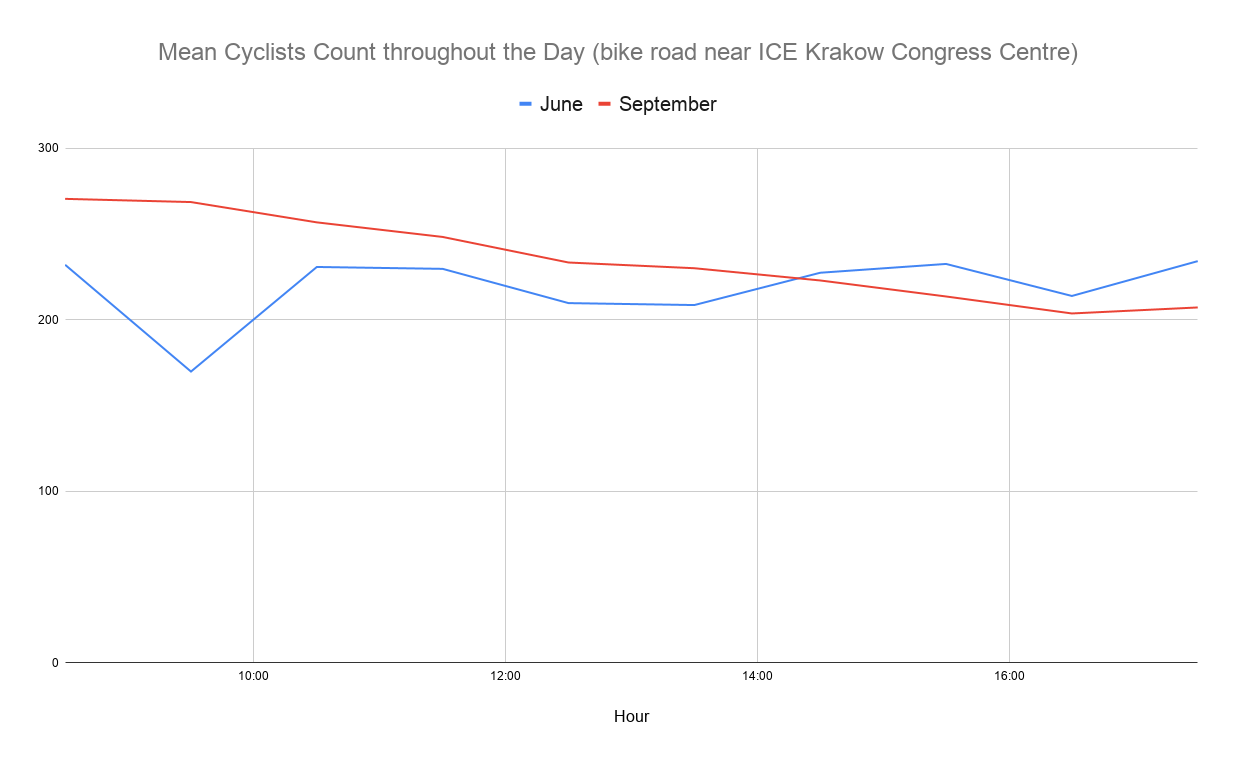
\includegraphics{images/graph4}}
    \caption{Cyclists count during the day - June to September comparison (bike road near ICE Krakow Congress Centre)}
    \label{fig:graph4}
\end{figure}
Figure \ref{fig:graph2} shows data from table \ref{tab:iceDaily} for easier comparison of results.
\begin{figure}[H]
    \centering
    \resizebox{\textwidth}{!}{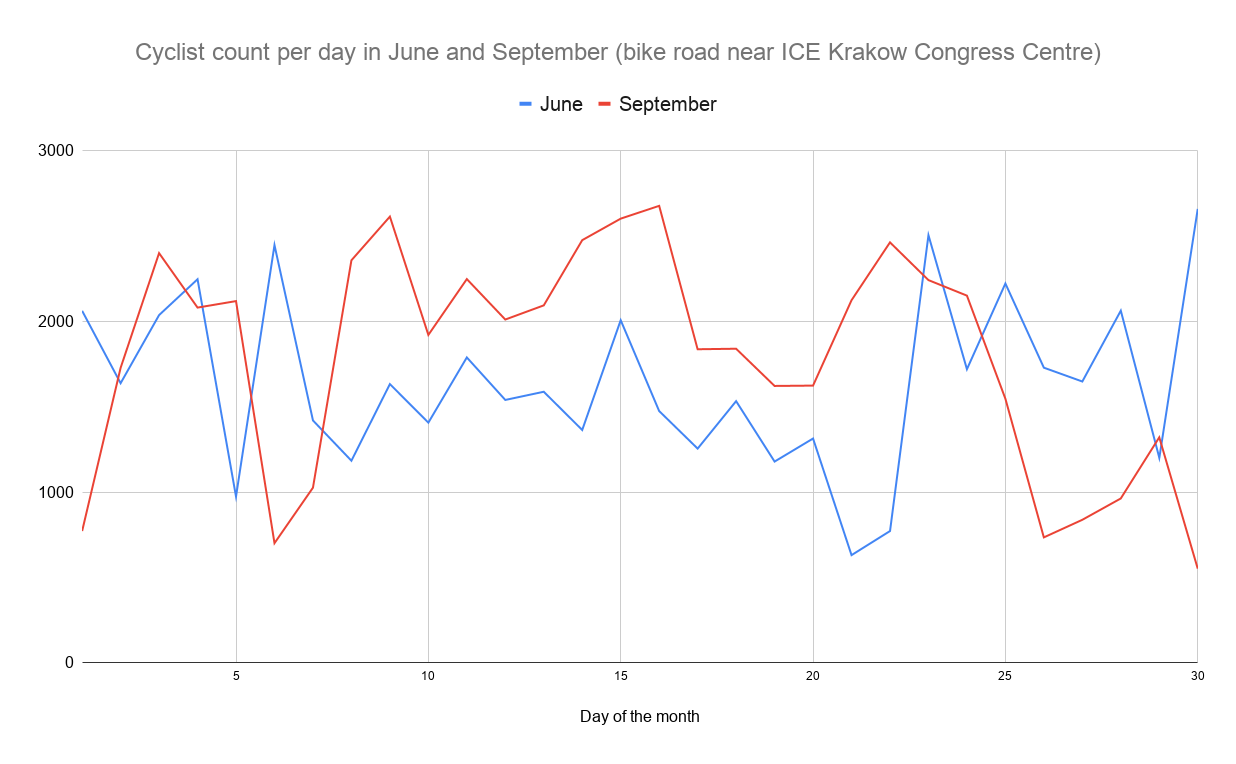
\includegraphics{images/graph2}}
    \caption{Cyclists count during the month - June to September comparison (bike road near ICE Krakow Congress Centre)}
    \label{fig:graph2}
\end{figure}
This simple example provides important information on how bicycle traffic changes on different months of the year. It shows if it grows or not. Various conclusions can be drawn. For example on figure \ref{fig:graph4} we can see that even though in September number of cyclists is higher that in June on early hours, it drops in later hours. After deeper analysis of different conditions those information can become a signal that maybe street lighting needs to be improved, considering that September is still quite warm month. It could be one of the ways to plan local government's projects. Second example shows different interpretation of similar data collected from camera on Lema Street where bike road was modernized. Table \ref{tab:lemaCount} show cyclists count during days of random week from July (before modernization) and October (after modernization). Table 
\begin{table}[h]
    \centering
    \resizebox{\textwidth}{!}{
    \begin{tabular}{|r|r|r|r|r|r|r|r|r|r|r|r|r|r|}
\hline
\multicolumn{7}{|c|}{Cyclists count throughout the day - July}                    & \multicolumn{7}{c|}{Cyclists count throughout the day - October}                     \\ \hline
09:45:00 & 10:45:00 & 11:45:00 & 12:45:00 & 13:45:00 & 14:45:00 & 15:45:00 & 09:45:00 & 10:45:00 & 11:45:00 & 12:45:00 & 13:45:00 & 14:45:00 & 15:45:00 \\ \hline
20       & 53       & 68       & 118      & 178      & 210      & 190      & 232      & 255      & 249      & 263      & 260      & 192      & 178      \\ \hline
229      & 261      & 180      & 386      & 210      & 305      & 436      & 419      & 291      & 311      & 424      & 353      & 216      & 259      \\ \hline
117      & 277      & 505      & 471      & 11       & 98       & 397      & 138      & 98       & 188      & 318      & 157      & 314      & 339      \\ \hline
118      & 385      & 92       & 315      & 350      & 121      & 290      & 390      & 499      & 271      & 373      & 104      & 212      & 61       \\ \hline
518      & 219      & 319      & 50       & 443      & 344      & 336      & 436      & 362      & 343      & 232      & 64       & 229      & 467      \\ \hline
293      & 179      & 130      & 171      & 49       & 27       & 12       & 485      & 519      & 331      & 242      & 118      & 97       & 41       \\ \hline
315      & 184      & 153      & 360      & 482      & 496      & 521      & 54       & 307      & 83       & 47       & 77       & 161      & 282      \\ \hline
\end{tabular}}
    \caption{Cyclist count during the day - week from July to week from October comparison (bike road on Lema Street)}
    \label{tab:lemaCount}
\end{table}
\begin{table}[h]
    \centering
    \begin{tabular}{|r|r|r|}
\hline
\multicolumn{1}{|l|}{}                & \multicolumn{2}{c|}{Cyclists count}                                \\ \hline
\multicolumn{1}{|l|}{Day of the week} & \multicolumn{1}{l|}{6-13 July} & \multicolumn{1}{l|}{5-12 October} \\ \hline
1                                     & 837                            & 1629                              \\ \hline
2                                     & 2007                           & 2273                              \\ \hline
3                                     & 1876                           & 1552                              \\ \hline
4                                     & 1671                           & 1910                              \\ \hline
5                                     & 2229                           & 2133                              \\ \hline
6                                     & 861                            & 1833                              \\ \hline
7                                     & 2511                           & 1011                              \\ \hline
\end{tabular}
    \caption{Daily cyclists count collected from street camera on Lema Street (sum of numbers for each day from table \ref{tab:lemaCount})}
    \label{tab:lemaSum}
\end{table}
Aggregation of this data for putting it on graphs like in first example:
\begin{figure}[h]
    \centering
    \resizebox{\textwidth}{!}{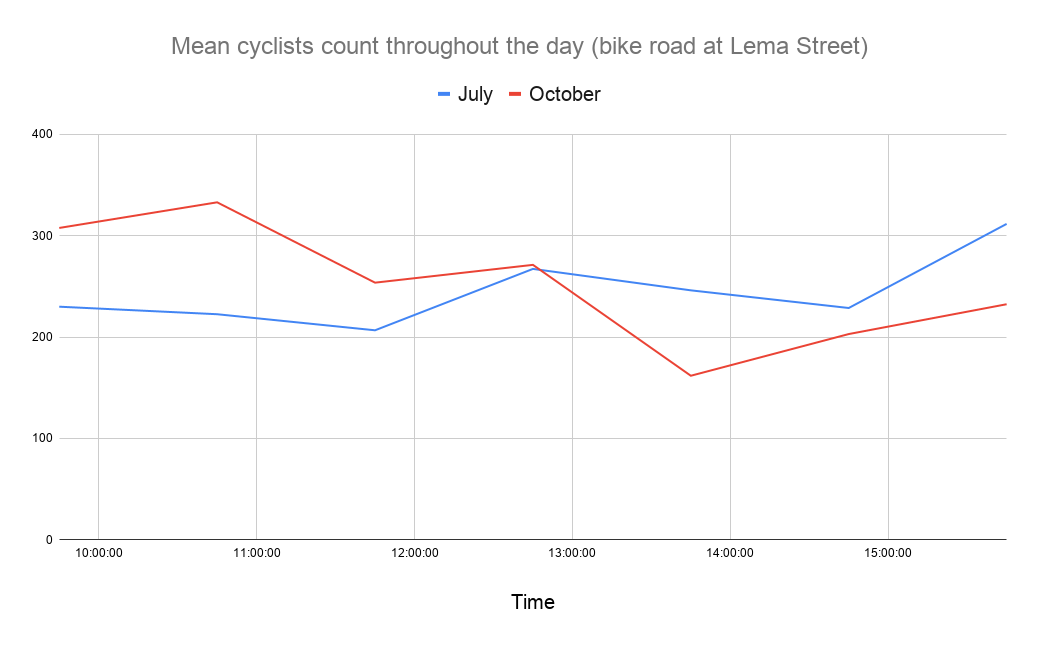
\includegraphics{images/graph6}}
    \caption{Weekly mean cyclists count on Lema Street for each hour - July to October comparison}
    \label{fig:lemaCount}
\end{figure}
\begin{figure}[h]
    \centering
    \resizebox{\textwidth}{!}{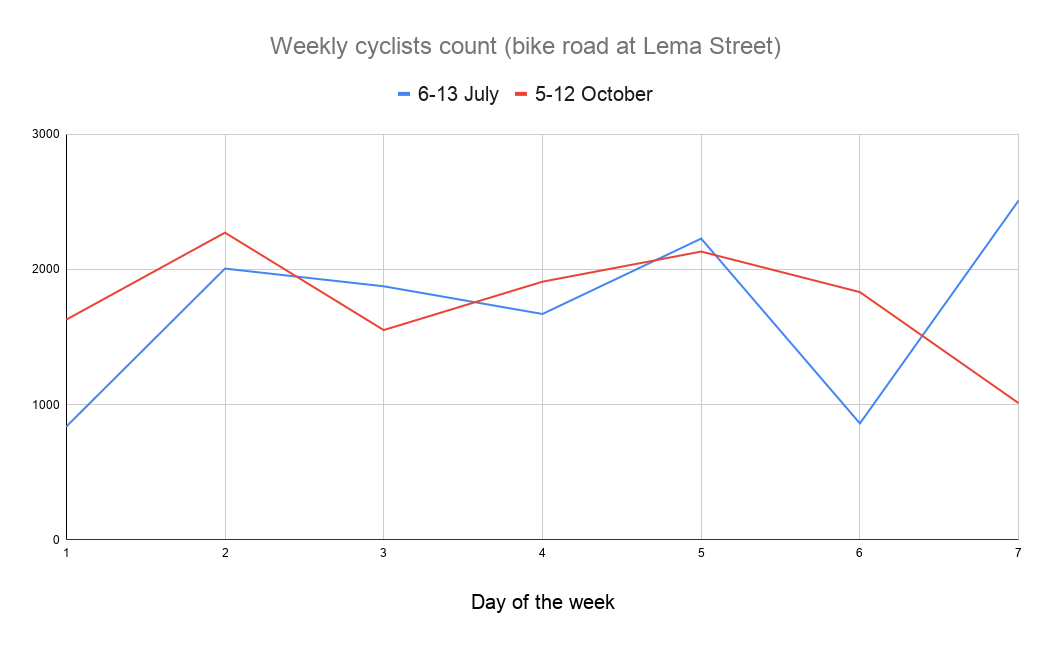
\includegraphics{images/graph5}}
    \caption{Cyclists count on Lema Street during chosen week - July to October comparison}
    \label{fig:lemaCount}
\end{figure}

Showing this data on a graph like in figures above won't show striking differences, but we can still see that overall more cyclists were detected in October than in July. There can be a lot of reasons why data looks like this, but collected numbers are very good indicators to compare with other parameters like weather conditions in specific month (temperature, rainfall level). Altogether it can serve as a tool for evaluation of made investments or for planning new ones.

\bibliographystyle{unsrt}
\bibliography{bibliography}

\end{document}
